\chapter{Background in Fault Detection, Isolation and Recovery}

In this chapter, we will discuss the theoretic fundamentals of Fault Detection, Isolation and Recovery (hereafter, ``FDIR"). We will look at how behavior of complex systems can be modeled in such a way that undesirable states can be clearly defined and detected. We will look at more modern, advanced techniques for this analysis. We'll also spend some time talking about analytical as well as human-centered issues with current techniques, in order to motivate the subsequent work within this thesis.

\section{Goals and Definitions}

First, we will define a handful terms in order to precisely discuss FDIR problems.

We will define a \textbf{fault} as any system state that is undesirable. When a fault is \textbf{detected}, a decision has been made that a fault has occurred. This will often by followed by an \textbf{alarm} step, in which the fault is made known to a human operator or to a higher level of a control system hierarchy. The process of fault \textbf{isolation} is a narrowing-down step in which the location, whether physical or logical, of a fault is determined \cite{schwabacher2008pre}. After a fault is isolated, the final step for an autonomous system is to \textbf{recover} from the fault, by returning to a non-faulty state or entering a ``safe" state in which the fault cannot negatively affect the system's ability to complete objectives. FDIR schemes for ensuring system safety are also referred to in the literature as ``fault protection" schemes \cite{kurien2010intrinsic}. A typical flow, including human interactive steps, is shown in \ref{fig:fp_flow}.

\begin{figure}[h]
\centering
    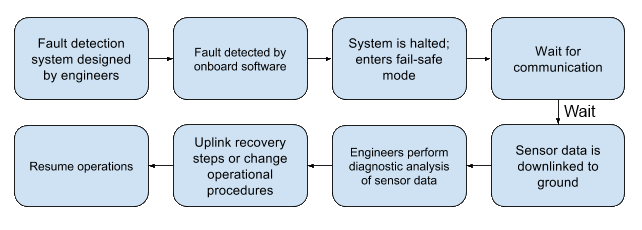
\includegraphics[width=\columnwidth]{images/fp_flow2.png}
    \caption{A typical fault detection flow. Adapted from \cite{kurien2010intrinsic}.}
    \label{fig:fp_flow}
\end{figure}

System behavior may be modeled as a finite state machine of \textbf{operational modes}, and system states are \textbf{monitored} or \textbf{telemetered} by sets of hardware sensors and software metrics, which inform the state of the system \cite{dearden2004real}. A system state or subset of values can be said to be \textbf{nominal} when it falls into a user-defined range of normal or safe operation; it can be described as \textbf{anomalous} when it does not. The term \textbf{out of family} is also used to describe data that is specifically anomalous for a certain operational mode.

System models may include ideal or expected behavior for a given operation mode, and a method for comparing the current state to the expected mode can be expressed as a \textbf{residual} \cite{hwang2010survey}, which is usually a measurement of a difference from a nominal state. Furthermore, faults can be divided into \textbf{fault levels}, often along the lines of a subsystem hierarchy or in terms of severity \cite{tipaldi2014spacecraft}.

\section{Model-Based FDIR}

Control systems for which FDIR is conducted are often represented with a modern state-space model, wherein plant dynamics are modeled as follows \cite{hwang2010survey}
\begin{equation} \label{eq:plant_model1}
    x(t+1) = A(t) x(t) + B(t) u(t) + E_{1}n_{1}(t),
\end{equation}
\begin{equation} \label{eq:plant_model2}
    y(t) = C(t) x(t) + D(t) u(t) + E_{2}n_{2}(t),
\end{equation}

where $x \in \mathbb{R}^{n}$ is the state vector, $u \in \mathbb{R}^{p}$ is the plant's input vector, $y \in \mathbb{R}^{m}$ is the sensor-measured output vector, $A$, $B$, $C$ and $D$ are realizations of linear dynamics with permissible perturbations, and $n_{1}$ and $n_{2}$ are disturbance vectors.

By observing the system via $y$, along with the known input $u$, it is possible to assess, via a model of expected system behavior, if the current state is an anomalous one. As discussed above, a measure of our deviation from this nominal state is the residual, and is commonly expressed as a difference between an estimated output $\hat{y}(t)$ and the observed output $y(t)$ \cite{hwang2010survey}, as follows:
\begin{equation} \label{eq:residual_generation}
r(t) = y(t) - \hat{y}(t)
\end{equation}

Note that many other residual generation algorithms are possible as well.

A block diagram illustrating how a residual generation system might be structured is shown in Fig.~\ref{fig:residual_block_diagram}.

\begin{figure}[h]
\centering
    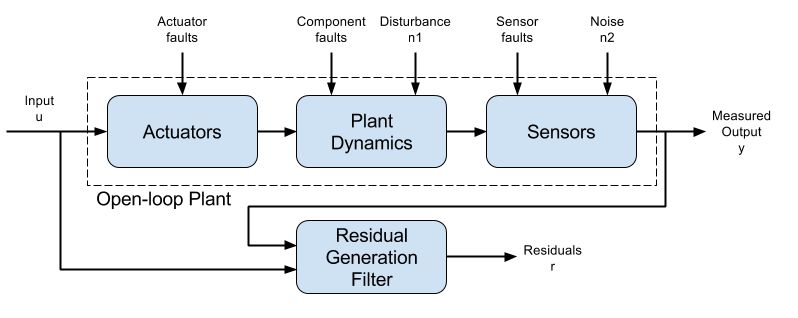
\includegraphics[width=\columnwidth]{images/residual_block_diagram2.png}
    \caption{A simple residual generation model for a dynamic system. Adapted from \cite{hwang2010survey}.}
    \label{fig:residual_block_diagram}
\end{figure}

Generated residuals can be evaluated via user-defined functions to assess whether a fault ought to be detected or not. The simplest form of fault residual comparison can be found in the setting of upper and lower bounds to describe the range of nominal values for a state. This ``threshold-based" system is the easiest variant of fault detection to implement, and is an important part of many modern FDIR systems \cite{walker1979fault}.

\section{Signal Processing-Based FDIR}

Signal analysis can also be used with particular types of dynamic systems in order to identify faults. Time-domain reflectometry, in which electrical line reflection is used to determine wiring integrity, is one such example \cite{lo2005noise}. This research will not look into applications of this type of FDIR.

% \section{Fault Filtering and State Observation}

% \subsection{Full-State Observer Fault Filters}

% \subsection{Parity-Space Filtering}

% \subsection{Kalman Filtering for FDIR}

% \cite{larson2002model}
% \cite{washington2000board}

% Also, particle filters:

% \cite{dearden2004real}

\section{Redundancy-Based Systems}

For systems that are difficult to model, such as complex software systems, redundant sensors and processing units may be used, under the suspicion of a fault being likely to occur in a single one of the redundant components. Parity-vector methods such as the Generalized Likelihood Test, or voting schemes such as Random Sample Consensus , may be used to isolate the components which are likely to be in error \cite{holsti2001towards}.

\section{Advanced Techniques for Fault Detection}

\subsection{Rule Combinations and Fault Syndromes}

Rule-based FDIR is an alternative to model-based FDIR in which a system-dynamic model, and predicted output values $\hat{y}(t)$, are not constructed, but instead, an expert system is used to make diagnostic decisions based on system output \cite{schwabacher2008pre}. The rule-based FDIR system uses a series of ``rules checks" to determine if the system state is an anomalous one for the current mode; often, this may consist of a combination of simultaneous tests, called a ``fault syndrome," whose passage or failure indicates the presence of an isolated fault \cite{hammett1991application}. Additionally, the rules may be structured as a decision tree or Bayesian network allowing for the diagnosis of a complex fault from a combination of simpler rules \cite{holsti2001towards} \cite{paakko2001bayesian}.

\subsection{Machine Learning and Classification}

Recent research has made progress into using machine learning techniques for classifying and identifying faults. An interesting overview of Support Vector Machines (SVMs) for FDIR is given in \cite{lin2006fault}, and \cite{aycard2000state} discusses the usage of Hidden Markov Models (HMMs) for a similar purpose.

This thesis will not attempt to examine these techniques in detail; however, it seems that they are likely to suffer from those problems typical of machine learning algorithms, including the necessity for a large amount of training data in order to learn nominal states, and the difficulty of human operator insight into the causes of anomalous states.

% \subsection{Distributed Fault Control}

% \cite{castel2006fdir}

\subsection{Common FDIR Issues and Motivations}

Many issues exist with traditional FDIR-based schemes which limit their utility.

One major issue is the likelihood of unmodeled errors to occur on any given complex system. FDIR systems designed by humans must rely on human understanding, and as such, unpredicted issues may arise where humans fail to anticipate all of the possible system failure modes. Research suggests that unmodeled faults are incredibly common in complex spacecraft systems, and thus, there is a need for other tools to capture anomalous system states \cite{kurien2010intrinsic}.

Another danger, especially relevant with expensive, teleoperated systems is the increased risk imposed by an automated recovery system. If a fault is detected and the system takes automatic action to recover, this action cannot be potentially harmful to the system. For faults that must be resolved immediately so as to not jeopardize a mission (such a thrust irregularities on a firing rocket), FDIR systems that preempt human decisions may be necessary, on longer timescales, the value of having human experts evaluate fault-suggestive data and manually decide how to proceed may outweigh the risks of autonomous recovery.

A detailed list of issues with model-based FDIR, with multiple references in the space industries and others, is given in \cite{kurien2010intrinsic}.

Because complex system faults, especially for teleoperated space systems, require large amounts of human analysis, creativity, and validation in order to understand root causes and recover from them, it is evident that the range of autonomous FDIR schemes is inadequate. We must create human-in-the-loop systems that augment model-based FDIR and analyze the resulting data to optimize the analytical work of root cause analysis and recovery.

In the next chapter, we will look at analysis techniques that help us examine behaviors of the system which we can visualize.